The program defines a two-qubit quantum circuit with two classical bits for measurement. It begins by applying Hadamard gates to both qubits to create a superposition of states. A controlled-$Z$ gate is then applied to introduce a conditional phase shift and generate entanglement between the qubits. Throughout the circuit, Hadamard and Pauli-$X$ gates are alternated to manipulate the amplitudes and phases of the quantum state, controlling its evolution step by step. A controlled-NOT ($CX$) gate further couples the two qubits, enabling conditional transformations based on the state of the control qubit. The \texttt{barrier} instructions are included to visually separate logical sections of the circuit without affecting the computation. Finally, the qubits are measured and the results are stored in the corresponding classical bits, allowing observation of the output in the computational basis. The command \texttt{qc.draw('mpl')} displays the schematic of the circuit, as it can be seen in \cref{fig:qiskit circuit}.

\vspace{0.5cm}
\begin{lstlisting}[language=Python, caption={Qiskit code}, label={lst:qiskit-circuit}]
import qiskit
from qiskit import QuantumCircuit, transpile
from qiskit_aer import AerSimulator
from qiskit.visualization import plot_histogram
import matplotlib.pyplot as plt
from qiskit.qasm3 import dumps

# step 0: create a Quantum Circuit
qc = QuantumCircuit(2, 2)  # 2 qubits, 2 classical bits

# step 1:<
qc.h(0)
qc.h(1)

# step 2:
qc.cz(1, 0)

# step 3:
qc.h(0)
qc.h(1)

# step 4:
qc.x(0)
qc.x(1)

# step 5:
qc.cz(1, 0)

# step 6:
qc.x(0)
qc.x(1)

# step 7:
qc.h(0)
qc.h(1)

# measure q[0] -> c[0]; measure q[1] -> c[1];
qc.measure(0, 0)
qc.measure(1, 1)

qc.draw('mpl')  # draw circuit diagram
\end{lstlisting}





\begin{figure}[H]
    \centering
    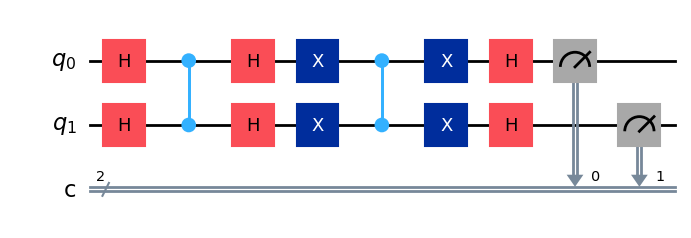
\includegraphics[width=0.7\textwidth]{images/circuit.png}
    \caption{Qiskit circuit}
    \label{fig:qiskit circuit}
\end{figure}


\begin{lstlisting}[language=Python, caption={Histogram with zero-count states}, label={lst:qiskit-hist}]
%matplotlib inline
from qiskit.visualization import plot_histogram

try:
    n_bits = len(next(iter(counts)))
except StopIteration:
    n_bits = getattr(qc, "num_qubits", 2)

labels = [format(i, f"0{n_bits}b") for i in range(2**n_bits)]
complete_counts = {b: counts.get(b, 0) for b in labels}

fig = plot_histogram(complete_counts, title="Measurements", bar_labels=True)
fig.show()
\end{lstlisting}

Through the previous code, the measurement results of the quantum circuit were visualized using a histogram, \cref{fig:output histogram}. The plot clearly shows that the only observed output is the bitstring \texttt{11}, while all other possible outcomes have zero probability. This indicates that the circuit deterministically evolves the quantum state into the final state $\ket{11}$, meaning that both qubits are measured in the state $\ket{1}$ with certainty.

\begin{figure}[H]
    \centering
    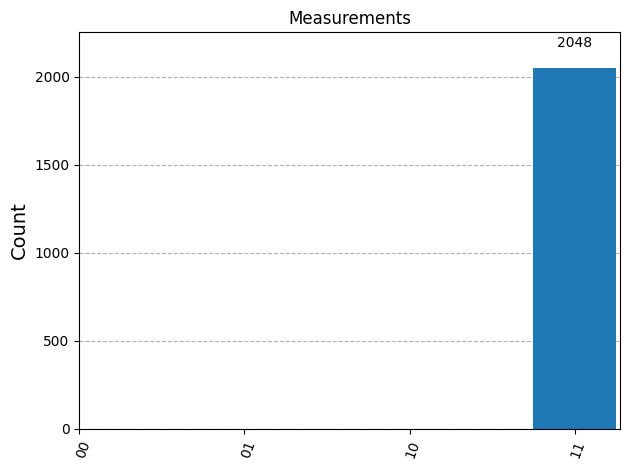
\includegraphics[width=0.7\textwidth]{images/histograms.png}
    \caption{output histogram}
    \label{fig:output histogram}
\end{figure}

%% Qasm 

The following two lines are used to convert the circuit into OpenQASM 3 code and display it:
\begin{lstlisting}[language=Python, caption={Export circuit to QASM3}, label={lst:qasm-export}]
qasm_str = dumps(qc)
print(qasm_str)
\end{lstlisting}

The first line serializes the circuit into QASM format, while the second prints the resulting code.

\begin{lstlisting}[language=Python, caption={Output generato: OpenQASM 3}, label={lst:qasm3-output}, backgroundcolor=\color{bg}]
OPENQASM 3.0;
include "stdgates.inc";
bit[2] c;
qubit[2] q;
h q[0];
h q[1];
cz q[1], q[0];
h q[0];
h q[1];
x q[0];
x q[1];
cz q[1], q[0];
x q[0];
x q[1];
h q[0];
h q[1];
c[0] = measure q[0];
c[1] = measure q[1];
\end{lstlisting}





